\chapter{Diseño e Implementación} % Main chapter title

\label{Chapter3} % Change X to a consecutive number; for referencing this chapter elsewhere, use \ref{ChapterX}
\definecolor{mygreen}{rgb}{0,0.6,0}
\definecolor{mygray}{rgb}{0.5,0.5,0.5}
\definecolor{mymauve}{rgb}{0.58,0,0.82}

\lstset{ %
  backgroundcolor=\color{white},   % choose the background color; you must add \usepackage{color} or \usepackage{xcolor}
  basicstyle=\footnotesize,        % the size of the fonts that are used for the code
  breakatwhitespace=false,         % sets if automatic breaks should only happen at whitespace
  breaklines=true,                 % sets automatic line breaking
  captionpos=b,                    % sets the caption-position to bottom
  commentstyle=\color{mygreen},    % comment style
  deletekeywords={...},            % if you want to delete keywords from the given language
  %escapeinside={\%*}{*)},          % if you want to add LaTeX within your code
  %extendedchars=true,              % lets you use non-ASCII characters; for 8-bits encodings only, does not work with UTF-8
  %frame=single,	                   % adds a frame around the code
  keepspaces=true,                 % keeps spaces in text, useful for keeping indentation of code (possibly needs columns=flexible)
  keywordstyle=\color{blue},       % keyword style
  language=[ANSI]C,					% the language of the code
  %otherkeywords={*,...},           % if you want to add more keywords to the set
  numbers=left,                    % where to put the line-numbers; possible values are (none, left, right)
  numbersep=5pt,                   % how far the line-numbers are from the code
  numberstyle=\tiny\color{mygray}, % the style that is used for the line-numbers
  rulecolor=\color{black},         % if not set, the frame-color may be changed on line-breaks within not-black text (e.g. comments (green here))
  showspaces=false,                % show spaces everywhere adding particular underscores; it overrides 'showstringspaces'
  showstringspaces=false,          % underline spaces within strings only
  showtabs=false,                  % show tabs within strings adding particular underscores
  stepnumber=1,                    % the step between two line-numbers. If it's 1, each line will be numbered
  stringstyle=\color{mymauve},     % string literal style
  tabsize=2,	                   % sets default tabsize to 2 spaces
  title=\lstname,                   % show the filename of files included with \lstinputlisting; also try caption instead of title
  morecomment=[s]{/*}{*/}%
}


%----------------------------------------------------------------------------------------
%	SECTION 1
%----------------------------------------------------------------------------------------
En el presente capitulo se realiza una explicación detallada de los módulos del hardware, tecnologías usadas, y el diseño e implementación del firmware.

\section{Módulos del sistema de hardware}

\subsection{Hardware}

En esta sección se explican todos los módulos de hardware que componen el prototipo del proyecto.

En la figura \ref{fig:Hierarchy} se puede observar la jerarquia del diagrama esquemático de todo el hardware.

\begin{figure}[h]
	\centering
	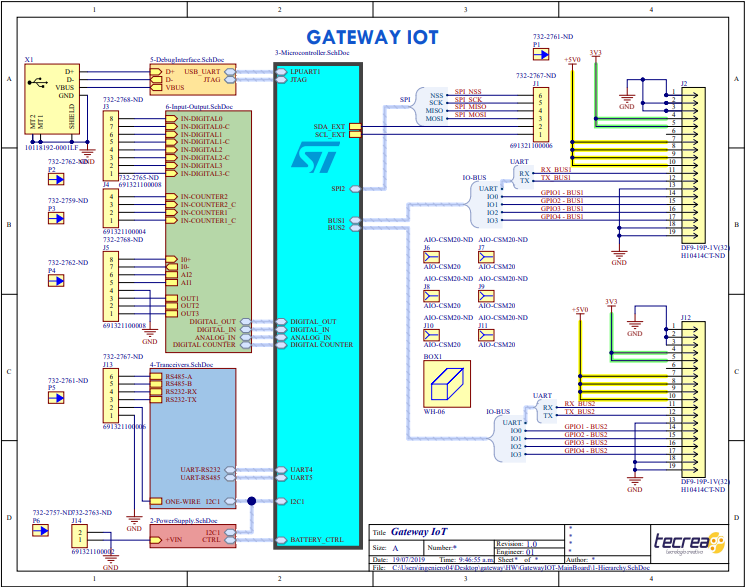
\includegraphics[scale=.65]{./Figures/Hierarchy.PNG}
	\caption{Jerarquia del hardware.}
	\label{fig:Hierarchy}
\end{figure}

\subsubsection{Microcontrolador}
A continuación se presentan las principales características del microcontrolador utilizado para el presente proyecto:
\begin{itemize}
    \item \textit{Ultra low power} ARM Cortex\textregistered-M4  CPU with FPU
    \item  SRAM 256 KB
    \item  Flash 1M
    \item 30 nA \textit{Shutdown mode (5 wakeup pins)}
    \item 120 nA \textit{Standby mode (5 wakeup pins)}
    \item 420 nA \textit{Standby mode with RTC}
   \item 3x I2C FM+(1 Mbit/s), SMBus/PMBus 
   \item 6x USARTs
   \item 3x SPIs
   \item 14-\textit{channel DMA controller}
    \item 16 x \textit{ timers}: 2 x 16-bit \textit{advanced motor-control}, 2 x 32-bit and 5 x 16-bit \textit{general purpose}, 2x 16-bit \textit{basic}, 2x \textit{low-power} 16-bit \textit{timers (available in Stop mode)}, 2x \textit{watchdogs, SysTick timer}
    \item \textit{Up to 114 fast I/Os, most 5 V-tolerant, up to 14 I/Os with independent supply down to 1.08 V}
\end{itemize}



\subsubsection{Modulo Sigfox}
Se decide escoger el modulo WISOL para la comunicación con la red Sigfox,  debido a que cumple con las especificaciones de poder comunicarse por UART y por que es muy económico, aproximadamente 3 USD en cantidades de miles. También por la disponibilidad en la bodega de componentes de Tecrea SAS.

El módulo para la comunicación Sigfox desarrollado por la empresa WISOL, opera en 2 zonas con frecuencia distinta, la cual puede ser configurable por software. Las principales características del módulo WISOL WSSFM11R2D\cite{Laboratory2001}  son las siguientes:
\begin{itemize}
    \item \textit{RF Frecuency} RC2 transmisión 902.2 MHz.
    \item \textit{RF Frecuency} RC2 recepción 905.2 MHz.
    \item \textit{RF Frecuency} RC4 transmisión 920.8 MHz.
    \item \textit{RF Frecuency} RC4 recepción 922.3 MHz.
    \item potencia de Transmisión 22.5 dBm.
    \item 2.5 uA en modo \textit{sleep}.
\end{itemize}

En la figura \ref{fig:SIGFOX_SCH} se observa el diagrama esquemático del hardware asociado al modulo Sigfox.

\begin{figure}[h]
	\centering
	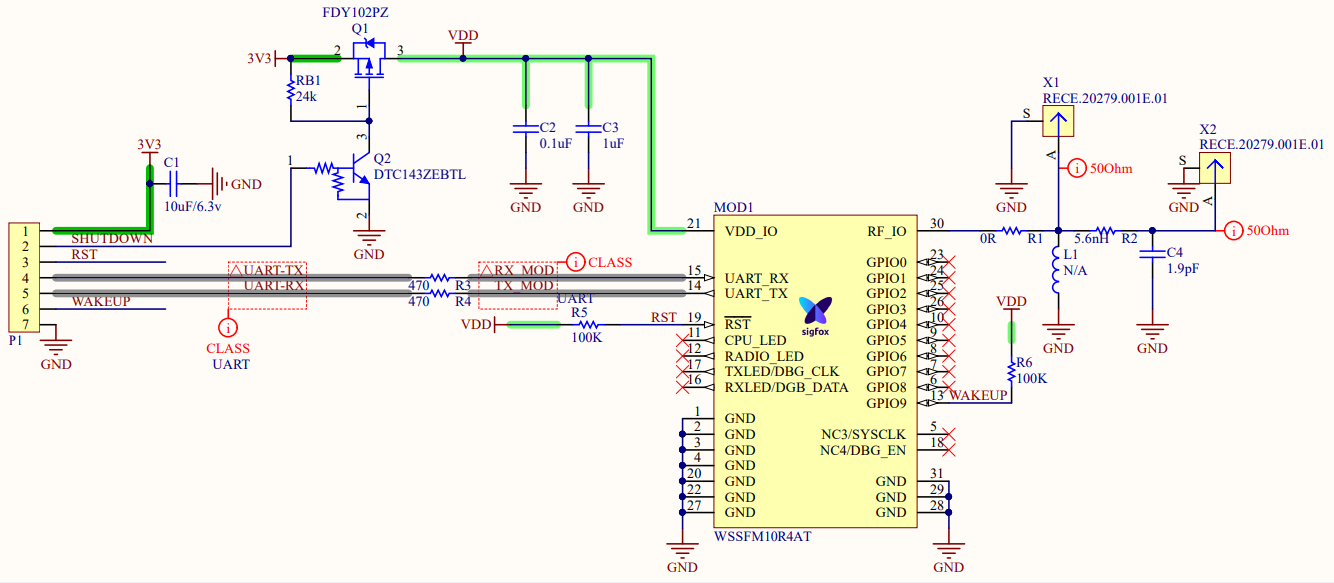
\includegraphics[scale=.4]{./Figures/SIGFOX_SCH.PNG}
	\caption{Esquemático módulo Sigfox.}
	\label{fig:SIGFOX_SCH}
\end{figure}

\subsubsection{Modulo Lora}
Se decide escoger el modulo LoRaWAN RN2903A para la comunicación, debido a que cumple con las especificaciones de poder comunicarse por UART y por que el costo es aproximadamente 12.05 USD en cantidades de miles y también por la disponibilidad en la bodega de componentes de Tecrea SAS.

El módulo para la comunicación LoRa, es fabricado por la empresa  Microchip Technology.
Las principales características del módulo RN2903A\cite{Range2018} clase A son las siguientes:
\begin{itemize}
    \item Opera en la banda de frecuencia de 915 MHz
    \item Modulación FSK, GFSK.
    \item 1.3 uA en modo \textit{sleep}.
    \item Potencia de Transmisión ajustable hasta 18.5 dBm.
\end{itemize}


En la figura \ref{fig:lORA_SCH} se observa el diagrama esquemático del hardware asociado al módulo LoRa.

\begin{figure}[h]
	\centering
	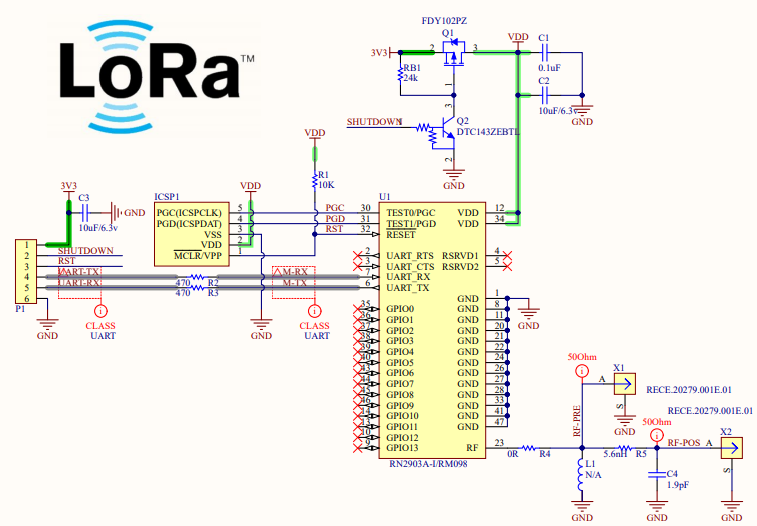
\includegraphics[scale=.55]{./Figures/lORA_SCH.PNG}
	\caption{Esquemático módulo LoRa.}
	\label{fig:lORA_SCH}
\end{figure}

Como el dispositivo esta enfocado al IoT, se garantizó desde la etapa de diseño que los módulos de las dos tecnologías consumieran lo mínimo posible en modo de bajo consumo, por lo que se implementó interruptores con transistores MOSFET (\textit{Metal-oxide-semiconductor Field-effect transistor}) en la alimentación principal de cada integrado.

\subsubsection{Entradas analógicas}

En la figura \ref{fig:inputanalog} se puede observar el diagrama esquemático de las entradas analógicas. Los valores de las resistencias se escogieron de acuerdo a los niveles de tensión y de corriente de las entradas (0-5VDC, 0-10VDC, 4-20mA) y el máximo voltaje permitido por el microcontrolador 3.3V. Todas las entradas analógicas tienen amplificadores en modo seguidor para acoplar impedancias y diodos TVS a la salida para garantizar los niveles de tensión máximo (3.3VDC).

\begin{figure}[H]
	\centering
	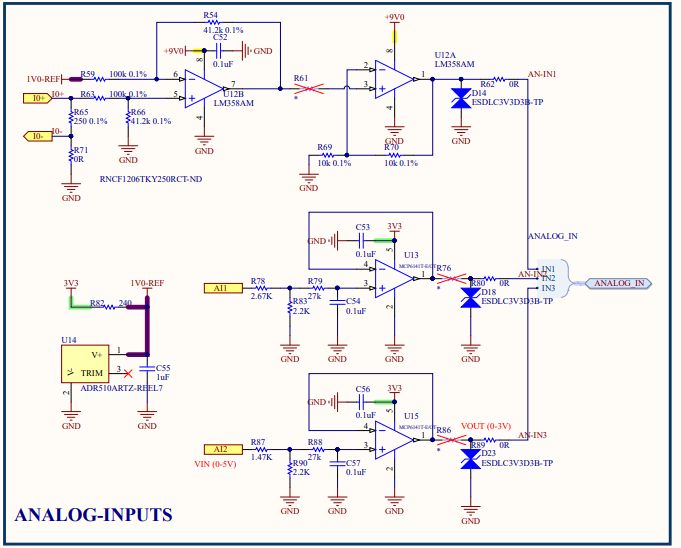
\includegraphics[scale=.65]{./Figures/inputanalog.PNG}
	\caption{Esquemático entradas analógicas.}
	\label{fig:inputanalog}
\end{figure}

\subsubsection{Entradas digitales}

En la figura \ref{fig:digitalinputs} se puede observar el diagrama esquemático de las entradas digitales, estas se encuentran opto-aisladas y funcionan con niveles de voltaje entre 3.3VDC a 24VDC.

\begin{figure}[H]
	\centering
	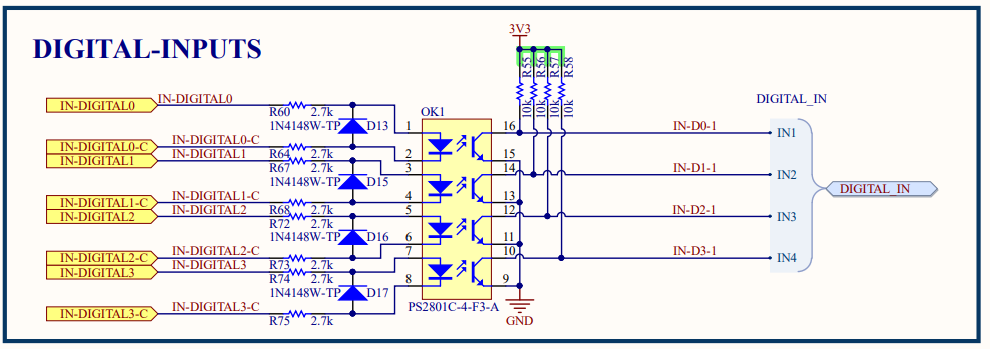
\includegraphics[scale=.45]{./Figures/digitalinputs.PNG}
	\caption{Esquemático entradas digitales.}
	\label{fig:digitalinputs}
\end{figure}

El modelo 3D y la tarjeta principal armada del prototipo se puede observar en la figura \ref{fig:mainboard} y \ref{fig:MainBoardCompleta}

\begin{figure}[H]
	\centering
	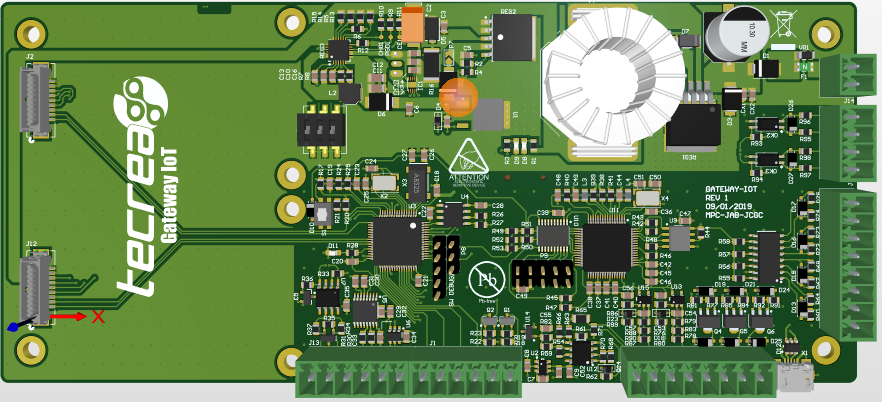
\includegraphics[scale=.45]{./Figures/mainboard3D.png}
	\caption{Modelo 3D tarjeta principal.}
	\label{fig:mainboard}
\end{figure}

\begin{figure}[H]
	\centering
	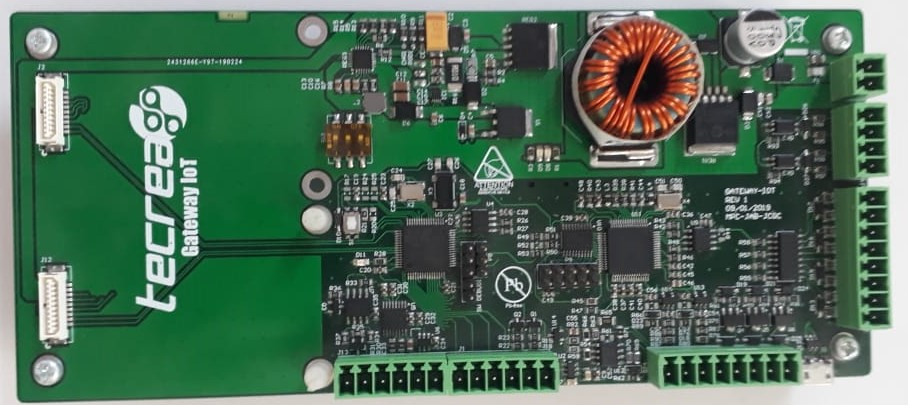
\includegraphics[scale=.45]{./Figures/mainboardSola.jpeg}
	\caption{Tarjeta principal ensamblada.}
	\label{fig:MainBoardCompleta}
\end{figure}
% Se puede agregar código o pseudocódigo dentro de un entorno lstlisting con el siguiente código:

% \begin{verbatim}
% \begin{lstlisting}[caption= "un epígrafe descriptivo"]

% 	las líneas de código irían aquí...
	
% \end{lstlisting}
% \end{verbatim}

% A modo de ejemplo:

% \begin{lstlisting}[caption=Pseudocódigo del lazo principal de control.]  % Start your code-block

% #define MAX_SENSOR_NUMBER 3
% #define MAX_ALARM_NUMBER  6
% #define MAX_ACTUATOR_NUMBER 6

% uint32_t sensorValue[MAX_SENSOR_NUMBER];		
% FunctionalState alarmControl[MAX_ALARM_NUMBER];	//ENABLE or DISABLE
% state_t alarmState[MAX_ALARM_NUMBER];						//ON or OFF
% state_t actuatorState[MAX_ACTUATOR_NUMBER];			//ON or OFF

% void vControl() {

% 	initGlobalVariables();
	
% 	period = 500 ms;
		
% 	while(1) {

% 		ticks = xTaskGetTickCount();
		
% 		updateSensors();
		
% 		updateAlarms();
		
% 		controlActuators();
		
% 		vTaskDelayUntil(&ticks, period);
% 	}
% }
% \end{lstlisting}


%-------------
%
%--------------


\subsection{Sintonización y verificación de la antena}
\label{subseccionAntena}
Tanto la red Sigfox como la red LoRa están dimensionadas para cubrir todo un territorio con una buena
calidad de servicio, tanto para aplicaciones interiores como exteriores. Incluso colocando los dispositivos en un entorno difícil u operando en los limites de la cobertura.
El rendimiento radiado de los dispositivos es fundamental para garantizar una buena conectividad. Los dispositivos que presenten un alto rendimiento radiado, obtendrán un beneficio completo de la red. Por lo tanto, la antena es un elemento clave en el diseño de un producto final, ya que es el componente que convertirá las señales conducidas en ondas electromagnéticas.

\subsubsection{Antena}
Es una estructura conductora en la que fluye una corriente eléctrica alterna (señal de RF (\textit{Radio Frequency})) generando campos eléctricos y electro magnéticos. La fuerza de esos campos dependen de la magnitud de la corriente eléctrica, pero también de la estructura de la antena\citep{AntenaSigFox2016}.

La sintonización de la antena en el presente trabajo se enfoca principalmente a la banda de la red Sigfox y LoRa. En el contexto de la tecnología Sigfox se debe seguir un procedimiento de certificación (\textit{Sigfox Ready\textsuperscript{TM}}), que garantiza la conformidad de un dispositivo en todas las condiciones operativas y durante el ciclo de vida completa. Esta certificación es obligatoria para cualquier dispositivo conectado a la red, con excepción de las soluciones de desarrollo. La certificación la realizan los laboratorio acreditados por Sigfox\citep{CertificationSigfox}.

En la certificación \textit{Sigfox Ready\textsuperscript{TM}} se mide la máxima potencia radiada efectiva ERP (\textit{Effective Radiated Power}) del dispositivo bajo prueba DUT (\textit{Device Under Test}) para definir la calidad del servicio y se tiene en cuenta la potencia radiada isotrópica efectiva EIRP (\textit{Effective Isotropic Radiated Power}) para las métricas de la certificación. El resultado de ERP se ve afectado principalmente por el diseño de la antena, ya que todos los circuitos integrados RF Sigfox trabajan con la misma potencia dependiendo de la zona de operación.

EIRP y ERP son parámetros de las antenas. Estos dependen de la potencia disponible en el puerto de la antena y describen cuánta potencia irradia un dispositivo en una dirección determinada. EIRP es la cantidad de potencia que una antena isotrópica necesitaría para irradiar la misma cantidad de potencia en una dirección dada como la antena medida\citep{Stutzman1981}. Mientras que ERP se refiere a una antena dipolo perfecta con una ganancia de 2.15dBi. Por lo tanto, la relación entre los valores de ERP y EIRP es simplemente un desplazamiento de 2.15dBi, como se describe en la siguiente ecuación \ref{eq:ERP_ECUA}.

\begin{equation}
	\label{eq:ERP_ECUA}
	ERPdBm = EIRPdBm - 2.15 
\end{equation}

\subsubsection{Carta de Smith}
La Carta de Smith ver figura \ref{fig:CartaSmith} es una ayuda gráfica para calcular las lineas de transmisión de circuitos de sintonización de antenas. Se utilizó para representar parámetros de impedancia (Z) en ohmios (\SI{}{\ohm}).

\begin{figure}[H]
	\centering
	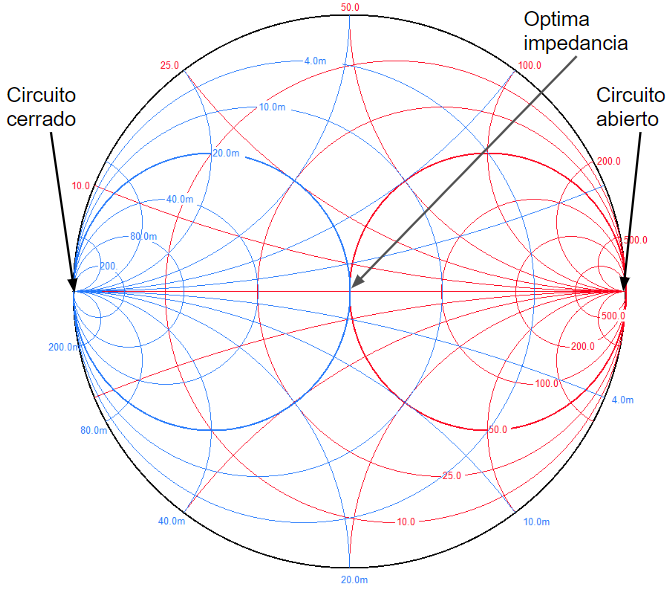
\includegraphics[scale=.45]{./Figures/CartaSmith.PNG}
	\caption{Carta de Smith.}
	\label{fig:CartaSmith}
\end{figure}
El manejo de la carta de Smith es fundamental, ya que basados en un punto de referencia se obtienen los valores aproximados de las bobinas y/o capacitores que se deben colocar en el circuito Pi (ver figura \ref{fig:cxPI}) que garanticen que la antena queda en la frecuencia adecuada y con la mejor eficiencia.
En la figura \ref{fig:ManejocartaSmith}  se puede observar como es el desplazamiento en la carta de Smith partiendo de un punto de referencia (impedancia). Comenzando del circulo azul del lado izquierdo, si se mueve el cursor hacia arriba o abajo se incrementa o decrementa el valor de la inductancia de la bobina que se debe colocar en serie en el circuito respectivamente. Partiendo del circulo rojo de en la parte derecha si se mueve el cursor hacia arriba o abajo se incrementa o decrementa el valor del capacitor en paralelo que se  debe colocar en el circuito Pi.

\begin{figure}[H]
	\centering
	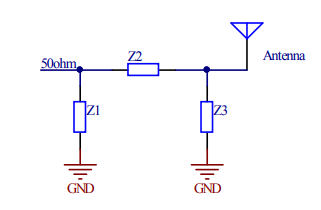
\includegraphics[scale=.65]{./Figures/cxPI.PNG}
	\caption{Circuito Pi\citep{NordicSemiconductor2012}.}
	\label{fig:cxPI}
\end{figure}

Al agregar un circuito Pi , que se compone de tres componentes paralelo, serie y paralelo como se puede observar en la figura \ref{fig:cxPI}, es posible cambiar la impedancia hasta 50 \SI{}{\ohm} (al menos con dos componentes) y se tiene la opción de que se puede realizar la sintonización en cualquier momento y para cualquier caso de uso. Es decir, si se tiene un dispositivo sintonizado para una aplicación especifica pero el mismo dispositivo se quiere usar para colocarlo por ejemplo, sobre una superficie metálica, simplemente se debería realizar la sintonización de nuevo y no afectaría en una nueva fabricación de PCB.
\begin{figure}[H]
	\centering
	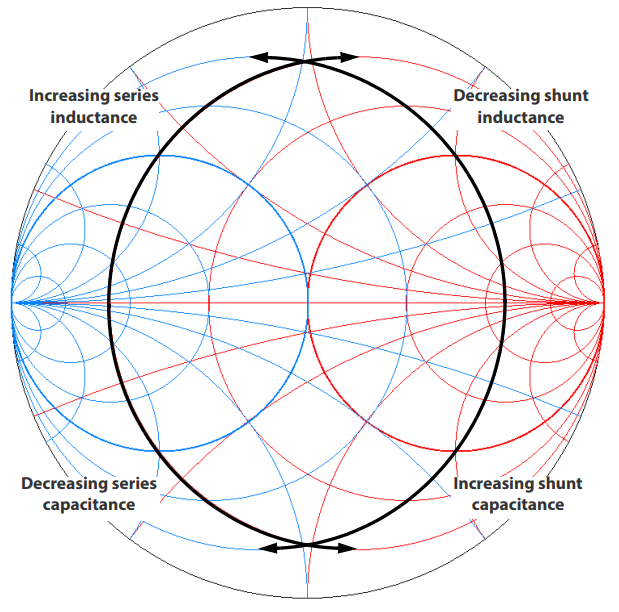
\includegraphics[scale=.45]{./Figures/ManejocartaSmith.PNG}
	\caption{Manejo carta de Smith\citep{NordicSemiconductor2012}.}
	\label{fig:ManejocartaSmith}
\end{figure}


\subsubsection{Consideraciones técnicas en el diseño de antenas}
A continuación se presentan algunas consideraciones técnicas para el diseño y/o sintonización de la antena:
\begin{itemize}
    \item El volumen de una antena delimita directamente su ancho de banda y eficiencia de radiación\citep{Gustafsson2007}. Por lo tanto, En las situaciones en que el espacio no sea una limitación, aumentar la superficie o el volumen de una antena permite aumentar su ancho de banda de impedancia\citep{TAntena2008}.
    \item Ubicación de la antena: la ubicación de una antena es crítica y tendrá un impacto en casi
    todos los parámetros de la antena. La mejor ubicación dependerá de la topología de la antena. No hay ley que lo determine\citep{CertificationSigfox}.
    \item Material de la carcasa: los materiales utilizados para fabricar la carcasa del dispositivo pueden ser críticos para el rendimiento de la antena. Esto es aún más crítico para las antenas pequeñas. Si las propiedades del material están disponibles, es mejor elegir un material con baja permitividad y pérdidas dieléctricas lo más bajas posibles. Plásticos como el ABS (\textit{Acrylonitrile Butadiene Styrene}) y la PC (\textit{Polycarbonates}) son muy son comunes y son materiales apropiados para la carcasa\citep{CertificationSigfox}.
    
    \item Carcasa metálica: en el caso de antenas integradas, la carcasa parcialmente metálica puede ser una opción, aunque la integración de la antena será más desafiante. En la mayoría de los casos, un metal. la carcasa tendrá que estar conectada al plano de tierra de la antena para evitar resonancias, que pueden conducir a una disminución en el rendimiento.  En el caso de las antenas integradas, se deben evitar las carcasas totalmente metálicas\citep{CertificationSigfox}.
    \item Componentes alrededor de la antena: la mejor manera de perturbar una antena es colocar un parte metálica al lado de la antena. El rendimiento puede verse afectado por una estructura metálica situada junto a la antena. Por lo tanto, es mejor evitar colocar componentes electrónicos grandes (por ejemplo, baterías, cámaras, altavoces) cerca de la antena, o tenerlos en cuenta al diseñar o sintonizar la antena. La disposición mecánica del dispositivo debe estar definida antes de la sintonización final de la antena (cualquier cambio tardío puede afectar la sintonización de la antena)\citep{CertificationSigfox}.
\end{itemize}
Estos pasos se deben seguir tanto en el prototipo como en el diseño final de la tarjeta y de la carcasa.

\subsubsection{Diferencias de desempeño presentado en las hojas de datos y en la vida real}
El rendimiento de la antena anunciado en las hojas de datos generalmente se aplica al diseño de referencia utilizado para caracterizar la antena. Por lo tanto, si el diseño del dispositivo con la antena integrada difiere de este diseño de referencia, es muy probable que el rendimiento que sea diferente. Dado que el diseño de referencia es probablemente el mejor para la configuración de la antena probada, debe esperar un rendimiento menor utilizando una implementación. Aquí hay una lista de parámetros que afectarán el rendimiento y el comportamiento de la antena en comparación con la hoja de datos inicial:

\begin{itemize}
    \item El tamaño de la PCB (\textit{Printed Circuit Board}) y los planos de tierra son bastante importante, ya que forma parte del mecanismo de radiación de la antena. La misma antena colocada en diferentes PCB no proporcionará el mismo rendimiento.
    \item La ubicación de la antena en la PCB también es un parámetro importante. Esto depende de los componentes y restricciones entre el plano de tierra y la antena, ver figura \ref{fig:chipantena}. Estas restricciones las define el fabricante y tienen gran impacto en la eficiencia de la antena.

\end{itemize}

\begin{figure}[h]
	\centering
	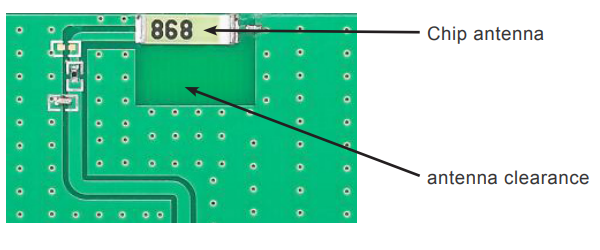
\includegraphics[scale=.35]{./Figures/chipantena.PNG}
	\caption{Restricción entre el plano de tierra y la antena.}
	\label{fig:chipantena}
\end{figure}
Es muy probable que el dispositivo tenga una carcasa que incluya todos los componentes electrónicos, incluida la antena, que probablemente no sea el caso con el diseño de referencia. Esta carcasa tendrá un impacto en la sintonización y la eficiencia de la frecuencia de la antena, según el tipo de material, su grosor y la distancia entre la antena y la carcasa. Idealmente, el material tan delgado y lo más alejado posible de la antena. Por supuesto,
esto no suele ser posible, por lo que aquí hay una lista de consejos enfocados a la realidad\citep{CertificationSigfox}:
\begin{itemize}
 \item Los plásticos con propiedades dieléctricas similares al ABS son aceptables. 
 \item Debe mantenerse una distancia mínima de 1-2 mm entre la antena y la carcasa.
 \item Debe respetarse un espesor máximo de plástico de 2 mm.
\end{itemize}

\subsubsection{Sintonización antena Sigfox} \label{subsectionSintonizar}
Sintonizar correctamente una antena mejora el rendimiento del transmisor. Si la antena no está correctamente sintonizada, se pierde mucha potencia del transmisor, se acorta el rango de operación y aumentan los problemas de interferencia.

La capacitancia y la inductancia de una antena están determinadas por sus propiedades físicas y su entorno. El parámetro más importante para la resonancia de la antena es la longitud. Una antena larga resuena a un menor frecuencia que una antena más corta porque la longitud de onda disminuye cuando la frecuencia aumenta. Esto significa que la longitud de la antena es directamente proporcional a la frecuencia y la longitud de onda\citep{NordicSemiconductor2012}.

Como la antena esta diseñada para una frecuencia especifica, su ancho de banda esta estrictamente limitado a esa frecuencia, una antena con frecuencia central 915 MHz y ancho de banda entre 902 a 928 MHz, como lo es Sigfox, no podrá trasmitir a 2.5 GHz. Una antena para poder aprovechar toda su eficiencia e irradiar al máximo debe resonar en su frecuencia de operación.

La frecuencia de resonancia es donde la impedancia de la inductancia XL es igual a la impedancia de la capacitancia XC , así que en la frecuencia de resonancia la antena es totalmente resistiva. 
% la reactancia inductiva (parte imaginaria de la impedancia de la bobina) es igual a la reactancia capacitiva (parte imaginaria de la impedancia %del condensador) 
Para un sistema óptimo, la impedancia en la antena debe coincidir con la impedancia del sistema que normalmente es 50 \SI{}{\ohm}.

Para la sintonización deben realizar los siguientes pasos :

\begin{itemize}
    \item Abrir la linea entre el modulo RF y la antena.
    \item Conectar la tarjeta a un VNA (\textit{Vector Network Analyzers}) por medio de un conector IPEX  a SMA, ver figura \ref{fig:VNATunnig}.
    \item Tener el dispositivo en el caso de uso.
    \item Analizar la carta de Smith y las perdidas de retorno y obtener el valor de la impedancia.
    \item Usar un programa para simular esta impedancia y poder moverse sobre la carta de smith y poder obtener los valores de los componentes.
\end{itemize}


\begin{figure}[h]
	\centering
	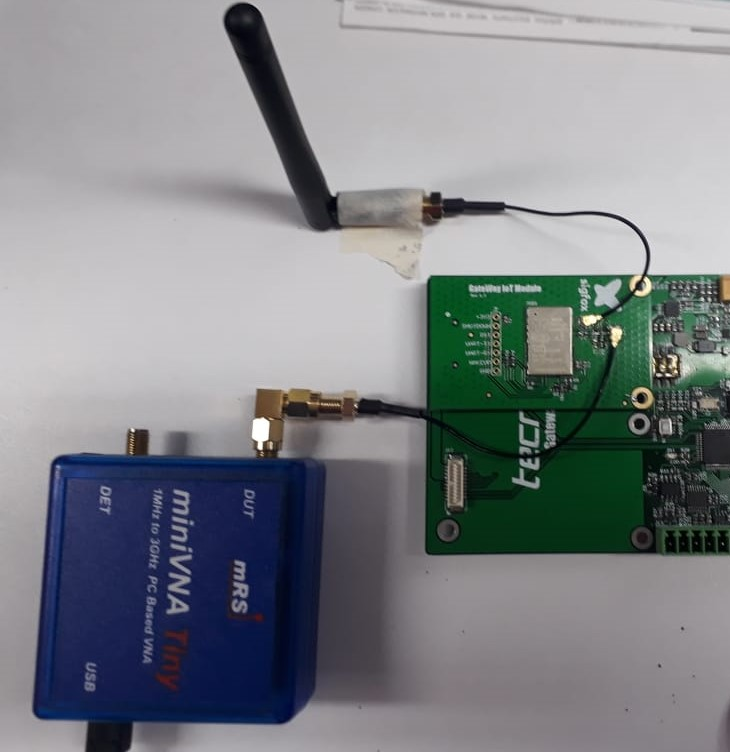
\includegraphics[scale=.45]{./Figures/VNATunnig.jpeg}
	\caption{Conexión Tarjeta con VNA.}
	\label{fig:VNATunnig}
\end{figure}

En el VNA se debe analizar que el marcador para la frecuencia de sintonización este lo mas cerca al origen donde la parte real de la impedancia es aproximadamente 50 ohmios y la parte imaginaria de la impedancia es 0, con esto se busca que exista lo menos posible perdidas de retorno. La perdida de retorno (Return Loss) es una relación entre niveles de potencia. En el puerto de la antena una parte incidente de la señal se refleja y otra es irradiada  o aceptada por la antena, entre menos reflexión haya mejor eficiencia tiene.

En la realidad es muy difícil tener una antena con el 100\% de la eficiencia, por lo que en la carta de Smith la impedancia debe estar en los alrededores del origen o en lo posible en el eje real, para que el dispositivo se considere sintonizado, también se debe analizar las perdidas de retorno la cual esta definida para Sigfox en -10dB \citep{AntenaSigFox2016}. Esta define el ancho de banda como se puede observar en la figura \ref{fig:returnlossTeorico}.

%
\begin{figure}[H]
	\centering
	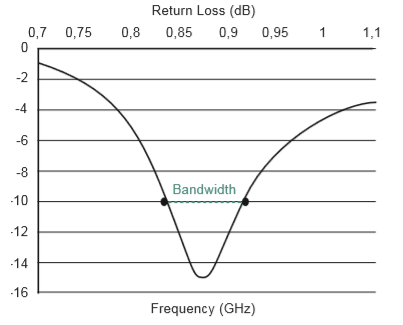
\includegraphics[scale=.6]{./Figures/returnlossTeorico.PNG}
\caption{Perdidas de retorno -10dB \protect\footnotemark.}
	\label{fig:returnlossTeorico}
\end{figure}

\footnotetext{\url{http://www.sigfox.com/en/resources/white-paper/antenna-design-essentials-for-sigfox-ready-tm-devices}} 


%e conoce como longitud de onda la distancia que recorre una perturbación periódica que se propaga por un medio en un determinado intervalo de tiempo
%0 dBd = 2,15 dBi “DBi” significa “ganancia de antena en dB por encima de un radiador isotrópico”; “DBd” significa “ganancia de antena en dB por %encima de una antena dipolo de media onda resonante”. 
%ERPdBm = EIRPdBm - 2.15 
%ERP is the parameter used in the SIGFOX device classification certification.
\subsection{Desarrollo del firmware}
% \subsection{Desarrollo de la capa de manejadores de dispositivos(\textit{driver}).}
 
 \subsubsection{Manejadores de dispositivos}
 Los manejadores de dispositivos son bibliotecas de código que permiten al sistema operativo interactuar con los periféricos haciendo una abstracción del hardware y proporcionando una interfaz para utilizar el dispositivo.
 
 Para el desarrollo de los manejadores de dispositivos, se usó el estilo de programación orientada objetos debido a lo practico que es encapsular y modularizar el código. % un objes to una clase es..... grafico
 
 \subsubsection{OS (\textit{Operating System}) QuarkTS}
Para el desarrollo del firmware del microcontrolador se usó un sistema operativo de tiempo real cooperativo llamado QuarkTS\cite{Camilo2019}. Se decidió trabajar con un OS (\textit{Operating System}) debido a que el planificador sigue un esquema orientado a eventos (Event Trigger System) e incorpora maquinas de estados vinculadas directamente a tareas  y esto ayuda a una mejor estructura del código y escalabilidad del proyecto. No se usó freeRTOS ni otros sistemas operativos \textit{open source}\protect\footnotemark por que dentro de las políticas de Tecrea SAS esta trabajar con el OS desarrollado por los ingenieros de la compañía. Esto siempre y cuando la aplicación lo permita, en caso de ser necesario se usan OS mas robustos como freeRTOS. Además se tiene un amplio soporte técnico , debido a que la persona que lo desarrollo trabaja  para la compañía y el OS se encuentra muy bien documentado.
\footnotetext{\url{https://www.osrtos.com/}}

Los estados de las tareas del QartkTS son cuatro: 
\begin{itemize}
    \item qWaiting: la tarea no se puede ejecutar porque las condiciones para la ejecución no están en lugar. En otras palabras, la tarea está esperando las condiciones para su ejecución.
    \item qReady: la tarea ha completado los preparativos para la ejecución, pero no puede ejecutarse porque se está ejecutando una tarea con mayor prioridad.
    \item qRunning: la tarea se está ejecutando actualmente.
    \item qSuspended : la tarea no participa en lo que está sucediendo. Normalmente el estado se toma después del estado qRunning o cuando la tarea no alcanza el qReady estado.
\end{itemize}
En la figura \ref{fig:TaskStateQartkTs} se puede observar el diagrama de flujo típico utilizado por QuarkTS para manejar los estados de las tareas. Está basado en el modelo Round-Robin, cada tarea se ejecuta desde la lista enlazada o cola de prioridades.
\begin{figure}[H]
	\centering
	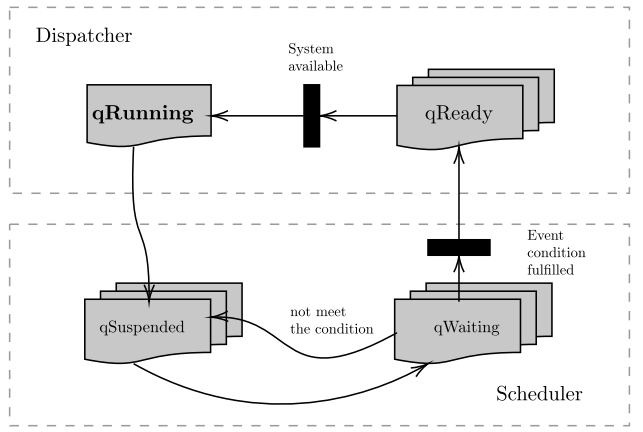
\includegraphics[scale=.65]{./Figures/TaskStateQartkTs.PNG}
	\caption{Estados de Tareas QuarkTS.\protect\footnotemark}
	\label{fig:TaskStateQartkTs}
\end{figure}
\footnotetext{\url{https://github.com/TECREA/QuarkTS/blob/master/quarkts-usermanual.pdf}}
 \subsubsection{Estructura del firmware}
 El firmware se estructuro de una forma que usara maquinas de estado finito y tareas disparadas por eventos. La máquina de estado es uno de los patrones de programación fundamentales. Los diseñadores usan este enfoque frecuentemente para resolver problemas complejos de ingeniería. Las máquinas de estado se compone en una serie de pasos finitos llamados estados. Cada estado realiza alguna función definida. Los eventos, por otro lado, son los estímulos que producen una transición entre estados.
El QuarkTS, Incorpora una maquina de estados a una tarea y desliga al programador de tener que realizarla como comúnmente se hace con un switch-case.

Cada máquina de estado tiene el concepto de estado actual (P). Este es el estado que actualmente ocupa la FSM. En cualquier momento dado, la máquina de estado puede estar en solo un estado. El estado de salida se puede manejar con subestados adicionales (S (b,s,u,f])) establecidos en el momento de la inicialización de FSM. Este flujo de trabajo entre el actual
estado y los subestados se muestran mejor en el gráfico \ref{fig:FSMQartkts}: 

\begin{figure}[H]
	\centering
	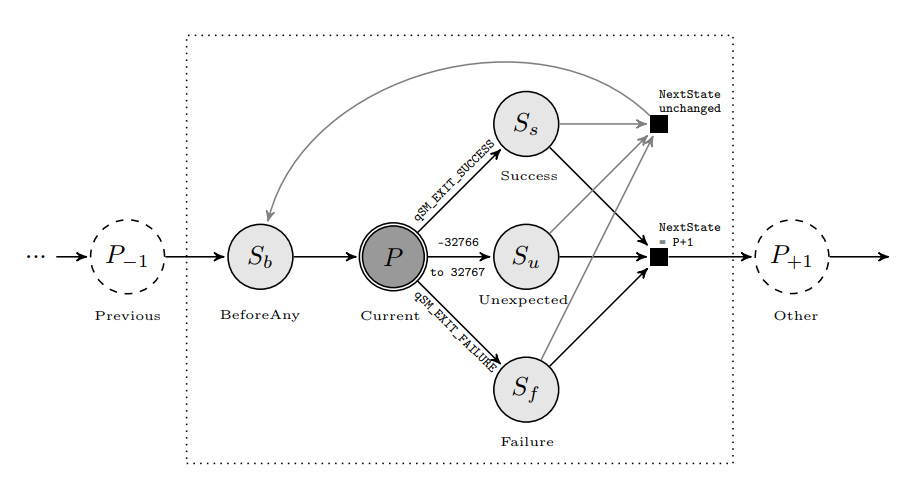
\includegraphics[scale=.65]{./Figures/FSMQartkts.PNG}
	\caption{Flujo de trabajo del OS QuarkTS.\protect\footnotemark}
	\label{fig:FSMQartkts}
\end{figure}
\footnotetext{\url{https://github.com/TECREA/QuarkTS/blob/master/quarkts-usermanual.pdf}}
La estructura del firmware se compone de cuatro tareas encargadas de :
\begin{itemize}
    \item Comunicación con el modulo Sigfox.
    \item Comunicación con el modulo LoRaWAN.
    \item Lectura de GPIO.
    \item Tarea para una FSM (\textit{Finite State Machine}).
\end{itemize}

%https://github.com/TECREA/QuarkTS/blob/master/quarkts-usermanual.pdf
El firmware se implemento con las tareas que se ven en el diagrama de la figura \ref{fig:Diagrama de flujo}.


%\begin{center}
\begin{figure}[!htb]
\centering
\begin{tikzpicture}[node distance=2cm]
\node (start) [startstop] {Scheduler};
%\node (in1) [io, below of=start] {lala};
\node (tSigfox) [process, left of=start, xshift=-2cm, yshift =-1.5cm] {tSigfox};
\node (tLoRa) [process, right of=start, xshift=2cm, yshift=-1.5cm] {tLoRa};
\node (dec1) [decision, below of=start, yshift=-0.1cm] {enQueue Payload};
\node (tIdle) [process, above of=tSigfox, yshift=0cm] {tIdle};
\node (tFSM) [process, below of=tLoRa, yshift= 0cm, xshift=0.5cm] {tFSM};
\node (tDisp) [process, below of=dec1, yshift=-1cm] {tDispPayload};


 \draw [arrow] (start) -- (tSigfox);
 \draw [arrow] (start) -- (dec1);
 \draw [arrow] (start) -- (tLoRa);
 \draw [arrow] (tSigfox) -- (dec1);
 \draw [arrow] (tLoRa) -- (dec1);
 \draw [arrow,dashed] (start) -- (tIdle);
 %\draw [arrow,dashed] (start) -| (tFSM.east);
 \draw [arrow] (tFSM.east) |- (start);
 \draw [arrow] (dec1) -- (tDisp);
\draw [arrow] (tDisp) -| (tFSM);
 

\draw [arrow] (dec1) -- node[anchor=east] {yes} (tDisp);
% \draw [arrow] (dec1) -- node[anchor=south] {no} (pro2b);

\end{tikzpicture}
\caption{Diagrama de tareas}
\label{fig:Diagrama de flujo}
\end{figure}

\subsubsection{Comunicación con el modulo Sigfox}
La tarea tSigfox se encarga de iniciar el servicio de comunicación con el módulo Sigfox, Le envía los comandos necesarios de configuración para dejarlo listo para trabajar, cuando se configura se deshabilita la tarea.

\subsubsection{Comunicación con el modulo LoRaWAN}
Esta tarea se encarga de iniciar el servicio de comunicación con el módulo LoRa, Le envía los comandos necesarios de configuración para dejarlo listo para trabajar, se basa en una corutina, cuando se configura se deshabilita la tarea.

\subsubsection{Lectura de entradas analógicas y digitales}
Esta tarea se encarga de muestrear periódicamente las señales analógicas y digitales.

\subsubsection{Despachador de mensajes}
Es una tarea que esta asociada a una cola de eventos. Esta tarea se dispara cada vez que hay un mensaje para transmitir en la cola.
\\
\newline
\newline
\newline
\newline
\hfill \break
\subsubsection{Tarea para una FSM (\textit{Finite State Machine})}
Esta tarea se encarga de realizar la secuencia de inicializar variables del sistema, enviar el mensaje por Sigfox o por LoRaWAN y colocar el módulo en modo de bajo consumo, la secuencia se repite periódicamente. En la figura \ref{fig:DiagramadeFSM} se puede observar la secuencia.

\begin{figure}[H]
\centering
\begin{tikzpicture}[node distance=2cm]
\node (start) [fsm] { Sleep };
%\node (in1) [io, below of=start] {lala};
\node (init) [fsm, left of=start, xshift=-2cm, yshift =-1.5cm] {  Init  };
\node (payload) [fsm, right of=start, xshift=2cm, yshift=-1.5cm] {Payload};

 \draw [arrow] (start) to [bend right=45] node[anchor=east] {Timeout} (init);
 \draw [arrow] (init) to [bend right=45]  (payload);
 \draw [arrow] (payload) to [bend right=45]  (start);



% \draw [arrow] (dec1) -- node[anchor=south] {no} (pro2b);

\end{tikzpicture}
\caption{Diagrama de la FSM}
\label{fig:DiagramadeFSM}
\end{figure}

